\subsection{Use Case 1: Enter symptoms}
\subsubsection{General Description}

\begin{tabular}{|p{.2\linewidth}|p{.65\linewidth}|}
\hline 
ID: & EnterSymptoms \\ \hline
Goal: & The user enters a description/keywords of their complaints for further analyzing. \\ \hline
Precondition: & - \\ \hline
Postcondition: & Get Diagnosis is executed. \\ \hline
Involved Users: &User: Someone who uses our system. \\ \hline
\end{tabular}

\subsubsection{UI to call the use case}
\begin{minipage}{0.4\textwidth}
\begin{figure}[H]
\centering
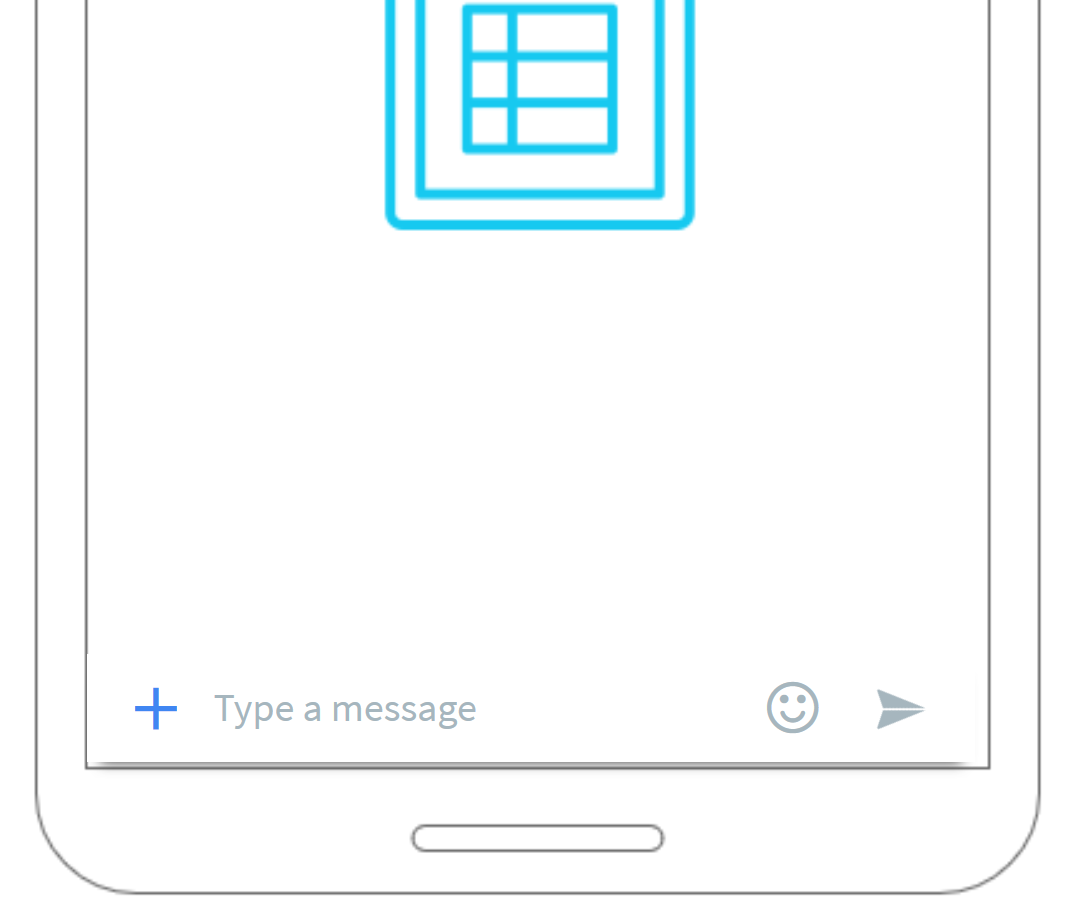
\includegraphics[scale=.4]{SystemSpec/Usecases/Mocks/entersym01.png}\\
\caption{\label{fig:blue_rectangle}enter symptoms}
\end{figure}
\end{minipage} \hfill
\begin{minipage}{0.6\textwidth}
The Dialog-Bar is used to describe your complaints and confirm said message.
\end{minipage}


\subsubsection{The Standard Use}
\begin{minipage}{0.4\textwidth}
\begin{figure}[H]
\centering
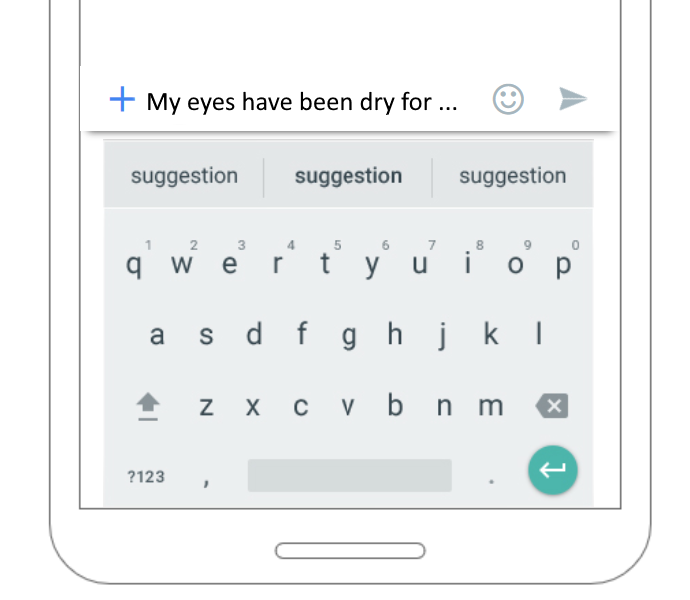
\includegraphics[scale=.27]{SystemSpec/Usecases/Mocks/entersym02Normal.png}\\
\caption{\label{fig:blue_rectangle}enter symptoms}
\end{figure}
\end{minipage} \hfill
\begin{minipage}{0.6\textwidth}
The user opens app, selects the Dialog-Bar enters his ailments into the app. Using words or whole sentences to describe the current malady.
\end{minipage}

\begin{figure}[H]
\begin{center}
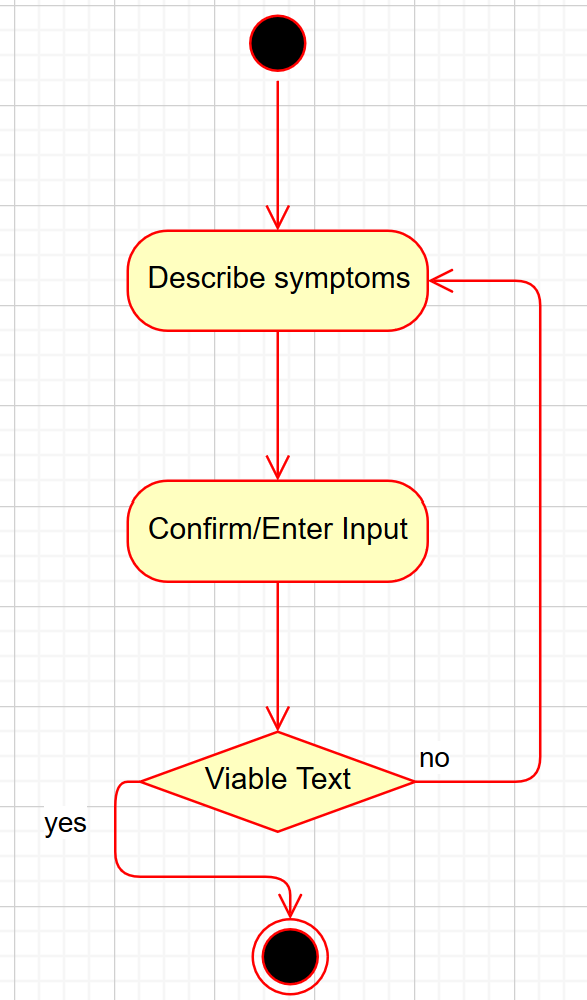
\includegraphics[scale=1]{SystemSpec/Usecases/Diagrams/entersymActivity.png}\\
\caption{\label{fig:blue_rectangle}enter symptoms}
\end{center}
\end{figure}

\subsubsection{The Non-Standard Use}
\begin{minipage}{0.4\textwidth}
\begin{figure}[H]
\centering
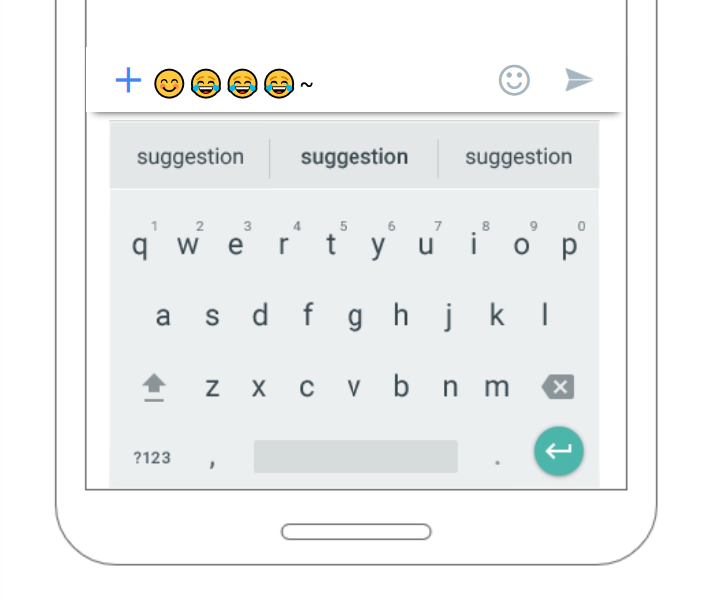
\includegraphics[scale=.7]{SystemSpec/Usecases/Mocks/entersym02Non.png}\\
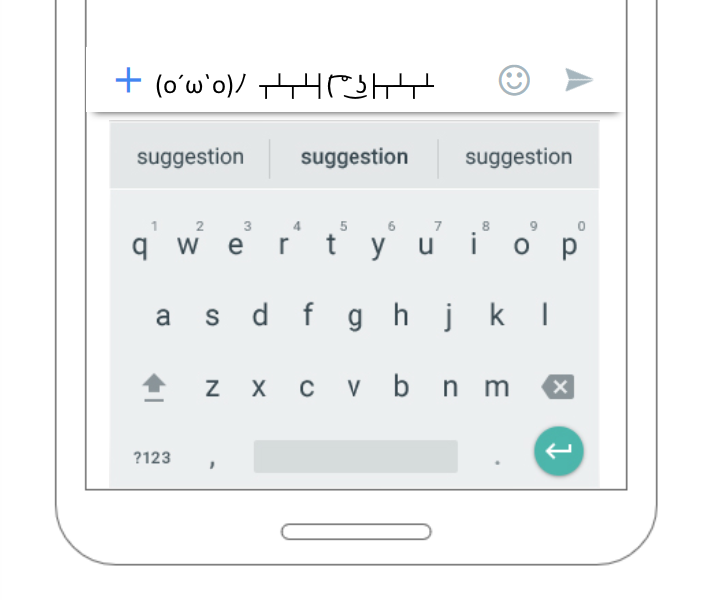
\includegraphics[scale=.7]{SystemSpec/Usecases/Mocks/entersym02NonAscii.png}\\
\caption{\label{fig:blue_rectangle}enter symptoms}
\end{figure}
\end{minipage} \hfill
\begin{minipage}{0.6\textwidth}
The user's input is not applicable. Before the input is transmitted to our back-end it will be checked for, for instance, senseless text like emojis or UNI-Code characters that are not used in languages. The input will be ignored and not further processed and the user will receive an error message.
\end{minipage}

\pagebreak
